\item
%\documentclass{beamer}
%\usepackage[utf8]{inputenc}
%\usepackage{amsthm}
%\usepackage{amsmath}
%\usepackage{graphicx}
%\usetheme{Madrid}
%\title{Control Systems (EE2227)}
%\author{Abhishek}
%\institute{IIT Hyderabad}
%\begin{document}
%\frame{\titlepage}
%\begin{frame}{Question}
Consider the following second order system with the transfer function:
\begin{multline}
G(s) = \frac{1}{1+2s+s^2}
\end{multline}
with input unit step 
\begin{multline}
R(s) = \frac{1}{s}
\end{multline}
 Let C(s) be the corresponding output. The time taken by the system output c(t) to reach 94\% of its steady state value, rounded off to two decimal places is
%\medskip
%\\ \hspace{20}(A)5.25\hspace{20}(B)4.50 \hspace{20}(C)3.89  \hspace{20}(D)2.81


%\end{frame}
%\begin{frame}{Answer}
%The approach for finding the solution is as follows:
%\begin{itemize}
 %   \item finding C(s)
  %  \item finding c(t)
   % \item finding the time at which c(t) attains 94\% of its steady state value
%\end{itemize}
%\end{frame}
%\begin{frame}{Finding C(s)}
%We are given G(s) and R(s), to find C(s), we can simply multiply these two

\textbf{Solution:}
\begin{multline}
C(s) = R(s).G(s) = (\frac{1}{s})  (\frac{1}{1+2s+s^2})
\end{multline}

\begin{multline}
C(s) =  \frac{1}{s(1+s)^2}
\end{multline}

%\end{frame}
%\begin{frame}{Finding c(t)}
%To find c(t), we have to do inverse Laplace transform on C(s)
%$$c(t) \longleftrightarrow C(s)$$
%Inverse Laplace transform can be calculated by the formula:
%$$f(t) = \frac{1}{2\pi j} \int_{a -j\infty}^{a+j\infty}F(s)e^{st} ds$$
%From the above formula, the inverse Laplace for some common expressions are:
%$$u(t) \longleftrightarrow \frac{1}{s}$$
%$$e^{-at} u(t) \longleftrightarrow \frac{1}{s+a}$$
%$$t e^{-at} u(t) \longleftrightarrow \frac{1}{(s+a)^2}$$
    
%\end{frame}
%\begin{frame}{Finding c(t)}

We found C(s) as:
\begin{multline}
C(s) =  \frac{1}{s(1+s)^2}
\end{multline}
%Now, we will use partial fractions to make applying Inverse Laplace easy.
%$$C(s) =  \frac{1}{s(1+s)^2} =  \frac{A}{s} + \frac{B}{(1+s)} + \frac{C}{(1+s)^2}$$
%We get, 
%\begin{align*}
%A &= 1 & A+B &=0 & 2A+B+C &= 0 \\
%A &=1 & B &=-1 & C &=-1
%\end{align*}
Therefore,
\begin{multline}
C(s) = \frac{1}{s} - \frac{1}{(1+s)} - \frac{1}{(1+s)^2}
\end{multline}
%\end{frame}
%\begin{frame}{Inverse Laplace}
%$$c(t) = L^{-1} ( \frac{1}{s} - \frac{1}{(1+s)} - \frac{1}{(1+s)^2}) $$
%From the properties of inverse Laplace transform,
%$$L^{-1} (F_1(s) + F_2(s) + F_3(s)) = L^{-1}(F_1(s)) + L^{-1}(F_2(s)) + L^{-1}(F_3(s))$$

Therefore;
\begin{multline}
c(t) = L^{-1} ( \frac{1}{s}) - L^{-1}(\frac{1}{(1+s)}) - L^{-1}(\frac{1}{(1+s)^2}) 
\end{multline}

Using the Known inverse transforms:
\begin{multline}
c(t) = (1 - e^{-t} - te^{-t}) . u(t)
\end{multline}

%\end{frame}
%\begin{frame}{Finding the time for reaching 94\%}


To know the steady state value of c(t), we calculate 
\begin{multline}
\lim_{t\to\infty} c(t) = (1+0+0).(1) = 1
\end{multline}

Now, 94\% of 1 is 0.94, so we should now solve for a positive t such that
\begin{multline}
(1 - e^{-t} - te^{-t}) = 0.94
\end{multline}
%the attached code gives us the solution for the equation
%and t turns out to be
\begin{multline}
 t = 4.5228
\end{multline}
%Therefore, answer is option (b)
%\end{frame}
%\begin{frame}{Plot}
%We can verify the solution by plotting c(t):
\begin{figure}
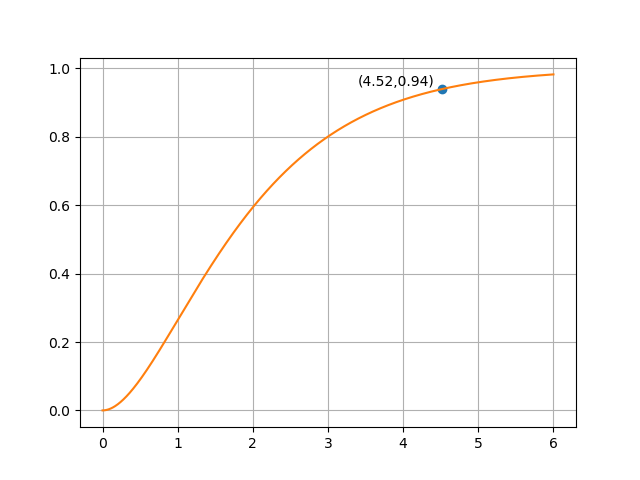
\includegraphics[scale=0.65]{./figs/plot.png}

\end{figure}
%\end{frame}    
%\begin{frame}{}
 % \centering \Large
 % \emph{THANK YOU}
%\end{frame}
%\end{document}
